\documentclass[10pt, twocolumn, a4paper]{article}

% Additional packages.
    \usepackage{graphicx}  % Images.
    \usepackage{esint}  % Additional integral symbols (eg: \iint).
    \usepackage[T1]{fontenc}  % Additional symbols (eg: \eth).
    \usepackage{multicol}
    \usepackage{float}
    \usepackage{hyperref}

% Margins.
    \usepackage[top=1cm, bottom=1.5cm, left=1cm, right=1cm]{geometry}
    \setlength{\columnsep}{1cm}
    \raggedbottom

% Space between paragraphs.
    \usepackage{parskip}
    % \setlength{\parskip}{11pt}

% Block break and word break.
    \hbadness=10000
    % \emergencystretch=\maxdimen
    % \hyphenpenalty=10000
    % \tolerance=1zz

% Title.
    \begin{document}
    \title{Sensor fusion on redundant angular rate sensors}
    \author{
        Author: Marcos Díaz
    }
    \date{
        Research period: 2021-2022\\
        Publication: November 2022\\
    }
    \maketitle

% Body.

\begin{abstract}
    It Is possible to improve angular rate sensor performance by combining data from multiple redundant sensors. Noise can be reduced by sampling each sensor in parallel, zero-rate can be reduced by opposing bias cancelling each other, and range can be extended without tradeoffs by configuring each sensor to different scales.
\end{abstract}

\section*{Acronyms}
    {\textbf{ARS}}: Angular Rate Sensor.\\
    {\textbf{DPS}}: Degrees Per Second.\\
    {\textbf{DTG}}: Dynamically Tuned Gyroscope.\\
    {\textbf{GPS}}: Global Positioning System.\\
    {\textbf{HID}}: Human Interface Device.\\
    {\textbf{IMU}}: Inertial Measurement Unit.\\
    {\textbf{PDF}}: Probability Density Function.


\section{Introduction}
    Redundant sensors (with equivalent characteristics) used in critical systems (aviation, medical) increase the reliability of the system in case of failure, but the individual characteristics of each sensor remain the same. \cite{sensor_failure_detection}

    In the other hand, is common to find multiple sensors of different nature used in consumer electronics, complementing each other to obtain better results (sensor fusion). An example of this is a smartphone combining {\textbf{GPS}} data and motion sensor data to reduce the uncertainty of location. \cite{adaptive_kalman}

    We will evaluate the possibility of using sensor fusion with redundant angular rate sensors to improve sensor performance (noise ratio, zero-rate and scale) in the domain of computer input.

\section{Problem}
    \subsection{Limitations of Angular Rate Sensors}
        As for today, most angular rate sensors available belong into two groups:

        Consumer electronics \textbf{IMU}s, sometimes with both accelerometer and {\textbf{ARS}} in a single chip, used in devices such as smartphones and videogame peripherals. These are based on the piezoelectric effect, are small, relatively inexpensive, and are energy efficient. Due to their small size, its performance characteristics (noise, zero-rate, scale) are limited, but enough for its intended uses such as smartphone tilt detection, step-counter, and mobile videogame input. \cite{piezo_mems}

        The next tier of motion sensor devices are industrial-grade or aerospace-grade, such as ring laser gyroscopes (Sagnac effect) and {\textbf{DTG}} rotor gimbals \cite{dtg}. These achieve very precise readings but are expensive and big, not suited for consumer electronics.

        Smartphone-grade IMUs prioritize small footprint and low energy consumption in their design, while performance characteristics such as noise ratio and zero-rate (drift) are only secondary. The miniaturized parts featuring the piezoelectric effect are prone to have high relative noise (compared with other common input methods such as a mouse optoelectronic sensor); and small variations in temperature cause an offset in their readings within a noticeable range.

        One of these novel application that require higher motion sensing performance than the provided by low-tier IMUs is Virtual Reality in the domain of videogames, in which aiming a (virtual) weapon is usually done by using both hands, each hand having an independent device featuring infrared spacial tracking, so the aim angle can be derived from the position of the hands in 3D space. On the contrary, aiming a pistol with a single hand must rely much more in single device angle detection, with much lower accuracy.

        Videogame controllers (Sony PlayStation DualShock, Steam Controller, Nintendo Switch Joy-Cons, etc...) have also been featuring motion sensors, but they were never used as a primary method for aiming (or other application that require very precise angular movements detection) due to the limitations of these smartphone-grade IMUs; and instead only using angular rate data as secondary input method to complement thumbstick or trackpad primary input for aiming.

    \subsubsection{Noise}
    \label{problem.noise}
        Noise is the unintended random disturbance on a signal. In commercially available ARSs noise is measured in $ mdps / \sqrt{Hz} $ (milli-degree per second by square root of frequency).

        Is not trivial to do a fair comparison with other common computer input methods such as mouse optoelectronic sensors, since these are a combination of camera and image processing hardware/software that effectively reduces noise to zero on the resulting output. \cite{optical_mouse}

        In practical terms, when using a optoelectronic sensor mouse for controlling a computer mouse cursor, noise is a non-factor; but when using a commercially available ARSs (using a reasonable {\textbf{DPS}} scale and operative system sensitivity) the noise can cause the mouse cursor to jitter several pixels back and forth at high frequency; making it unfit for the purpose unless applying filtering techniques with significant tradeoffs in latency (smoothing) or linearity (acceleration).

        Common solutions for reducing noise are:
        \begin{itemize}
            \item Frequency filtering: Either via hardware or software, to reduce the amplitude of undesired frequencies. Usually removing frequencies that are much higher or much lower than what the user is expected to input as real signal. By definition cannot remove noise in the frequency range of real input, or it would be filtering out such input.
            \item Multisampling: Since noise is a random value within a range, averaging the value of samples over time approximate the result to zero, the more samples the more reduction of noise, but with the tradeoff of increased latency, which is also an undesired attribute for videogame input.
            \item Acceleration: By applying an exponential response curve, the parts of the signal with low amplitude are reduced further, including noise. In applications in which linearity is required to achieve consistent results (as is videogame input), this is a undesired tradeoff.
            \item Sensor fusion: Using a secondary sensor of different nature to discard noise more effectively, each sensor have noise with its own characteristics, but the combination of data from both can help to isolate real input from unintended input.
        \end{itemize}

    \subsubsection{Scale}
        Angular rate sensors have a limit in the turn rate they can report on. These are also measured in maximum DPS until they saturate its data channel. For commercially available ARSs this attribute can be configured, usually in predefined steps from 125 DPS to 4000 DPS, referred as ranges or scales.

        There are tradeoffs depending in which scale to choose, smaller scales have better granularity (lower DPS per Least Significant Bit), better noise-signal ratio, and smaller zero-rate ratio, but can only report on slower turns. On the contrary, bigger scales have worse granularity, worse noise-signal ratio, an greater zero-rate, but they can report on faster turns.

        Since noise and zero-rate in ARSs are not negligible, these tradeoffs can be problematic no matter the chosen scale.

        One potential solution is to change the scale dynamically when the current range is too small or too big. But such request to the IMU is relatively slow and a blocking operation, so no reading from the sensor can be taken while the scale is being adjusted. Therefore this method cannot be employed if the system is expecting continuos readings with a smaller interval than the time it takes to change the scale.

    \pagebreak
    \subsubsection{Zero-rate}
        Zero-rate (also known as random walk offset or drift) \cite{zero_rate} is a deviation over time of the calibrated zero, doing a pseudo-random walk around the real zero at a much lower frequency than flicker noise (section \ref{problem.noise}). In piezoelectric-based IMUs this can be caused by electrical current instability, interference from other electronic components, or subtle changes in temperature.

        Zero-rate is measured in maximum DPS of deviation the sensor could reach away from the calibrated zero, and DPS/Cº for changes in temperature. For commercially available ARSs these are in the range of milli-degrees per second, but aggregated over time these can lead to much greater values.

        For the application of computer input, this is a big shortcoming of ARSs compared with alternative methods such as optical mouse, which similarly to noise (section \ref{problem.noise}), they have inexistent or negligible drift.

        Common solutions for zero-rate are:
        \begin{itemize}
            \item Acceleration: By applying an exponential response curve, the parts of the signal with low amplitude are reduced further, including noise. In applications in which linearity is required to achieve consistent results (as is videogame input), this is a undesired tradeoff.
            \item Multisampling: Contrary to the case of flicker noise, averaging multiple samples \textbf{of the same sensor} over time would NOT reduce zero-rate, since zero-rate is random-walk noise, consecutive values will contain very similar deviation, making multisampling useless.
            \item Self-correction: With software, when a constant angular rate is detected for several consecutive seconds, can be assumed it is not real input and the sensor can be programmatically calibrated.
        \end{itemize}

\pagebreak
\section{Redundant sensor fusion}
    \subsection{Noise}
        By using multiple physically connected sensors, is possible to take samples in parallel and average their values without increasing latency.

        The following figures show a sinusoidal representing actual input, with added simulated noise (normal distribution loc=0 scale=0.5), being processed with different combinations of multisampling and multisensor. Latency being defined as:

        $$ Latency = \frac{Samples}{Sensors} $$

        Figure \ref{fig_noise_1} shows the untreated signal on a single sensor.
        \begin{figure}[H]
            \caption{Sensors=1, Samples=1, Latency=1}
            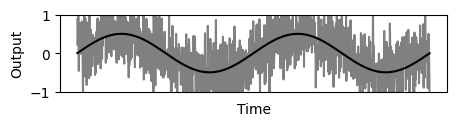
\includegraphics[width=\linewidth]{figure_noise_1.png}
            \label{fig_noise_1}
            $$ f_1(x) = sin(x) + N(\mu=0, \sigma=1) $$
        \end{figure}
        \vspace{-4mm}

        Figure \ref{fig_noise_2} shows result of multisampling method over 4 samples, significantly reducing the noise, but increasing latency.
        \begin{figure}[H]
            \caption{Sensors=1, Samples=4, Latency=4}
            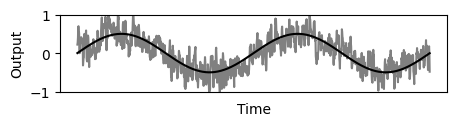
\includegraphics[width=\linewidth]{figure_noise_2.png}
            \label{fig_noise_2}
            $$ Avg(x, t) = \frac{ \sum_{x}^{x+t-1}f_1(x) }{t} $$
            $$ f_2(x) = Avg(x,4) $$
        \end{figure}
        \vspace{-4mm}

        Figure \ref{fig_noise_3} shows equivalent noise reduction (using a second sensor signal) but with improved latency. Note that the signal is not just scaled down version of the original noise, but also shows features (relative peaks) of the second sensor averaged signal.
        \begin{figure}[H]
            \caption{Sensors=2, Samples=4, Latency=2}
            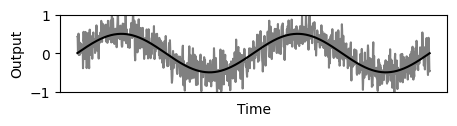
\includegraphics[width=\linewidth]{figure_noise_3.png}
            \label{fig_noise_3}
            $$ f_3(x) = \frac{Avg(x_1,2) + Avg(x_2,2) }{2} $$
        \end{figure}
        \vspace{-4mm}

        Figure \ref{fig_noise_4} shows improved noise reduction by using 2 sensors given the same latency as figure \ref{fig_noise_2}.
        \begin{figure}[H]
            \caption{Sensors=2, Samples=8, Latency=4}
            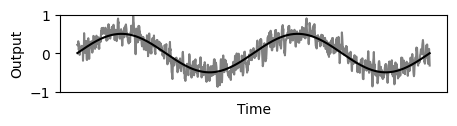
\includegraphics[width=\linewidth]{figure_noise_4.png}
            \label{fig_noise_4}
            $$ f_4(x) = \frac{Avg(x_1,4) + Avg(x_2,4) }{2} $$
        \end{figure}
        \vspace{-4mm}

        Figure \ref{fig_noise_5} shows further improvement of noise reduction by using 3 sensors given the same latency as figure \ref{fig_noise_2}.
        \begin{figure}[H]
            \caption{Sensors=3, Samples=12, Latency=4}
            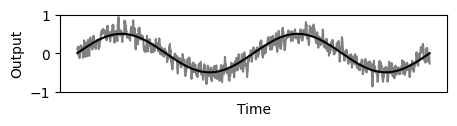
\includegraphics[width=\linewidth]{figure_noise_5.png}
            \label{fig_noise_5}
            $$ f_5(x) = \frac{Avg(x_1,4) + Avg(x_2,4) + Avg(x_3,4) }{3} $$
        \end{figure}
        \vspace{-4mm}

        The conclusion is that redundant sensors (of equal or similar characteristics) can be used to either reduce total noise more effectively within the same latency, or to achieve the same level of noise reduction but with less latency.

        The benefits of parallelism regarding latency does scale linearly with number of redundant sensors as $latency/n$ (there are no diminishing returns of using more than 2 sensors); while benefits regarding noise reduction only increase at a $1/n$ rate, so there are diminishing returns when adding more sensors.

    \subsection{Scale}
        While changing the scale dynamically with a single sensor is problematic (see section \ref{problem.noise}), it is possible to obtain the same multi-scale benefits with multiple sensors without these tradeoffs. By using multiple sensors, each one permanently adjusted to a different scale, then using the output of the most suitable sensor (the one with the smaller scale able to fit the input without saturate) a result with lower noise and lower zero-rate is obtained when the input is small, but without limitations in range when the input is greater.

        Given a system with multiple sensors $ S_n $, each sensor with a range $R_n$, and sorted from greater to smaller range, the final output can be defined as:

        $$
            Output =
            \cases{
                if(S_1 > R_2) \rightarrow S_1 / R_1 \cr
                else \: if(S_2 > R_3) \rightarrow S_2 / R_2\cr
                ... \cr
                else \: if (S_{n} > R_{n+1}) \rightarrow S_{n} / R_n \cr
                ... \cr
                else(S_n / R_n)
            }
        $$

        \pagebreak
        In the following figures an increasing $sin(x)$ function is representing actual input, then noise is used to visualize the undesired characteristics which are relative to the used scale (noise, zero-rate) in the values for the sensors $A$ and $B$

        \begin{figure}[H]
            \caption{Actual input}
            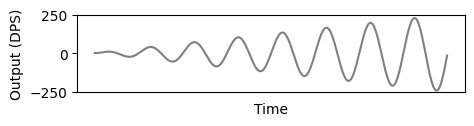
\includegraphics[width=\linewidth]{figure_scale_1.png}
            \label{fig_scale_1}
        \end{figure}
        \vspace{-8mm}

        Sensor $A$ is able to fit the full amplitude of the input, but noise is greater than in sensor $B$.
        \begin{figure}[H]
            \caption{Sensor A, scale=250}
            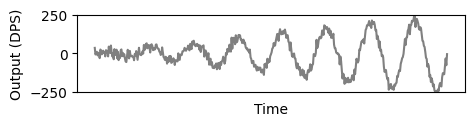
\includegraphics[width=\linewidth]{figure_scale_2.png}
            \label{fig_scale_2}
        \end{figure}
        \vspace{-8mm}

        Sensor $B$ noise is relatively smaller, but the input signal makes it to saturate after a certain point.
        \begin{figure}[H]
            \caption{Sensor B, scale=125}
            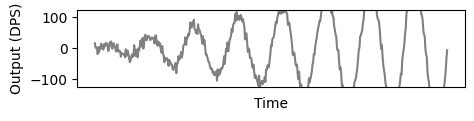
\includegraphics[width=\linewidth]{figure_scale_3.png}
            \label{fig_scale_3}
        \end{figure}
        \vspace{-8mm}

        Using the method described above the last figure shows how values of $B$ (with less noise) are used while the signal does not saturate it. But when sensor $B$ starts saturating it switches to the values of sensor $A$, which is able to capture the full amplitude of the real input.
        \begin{figure}[H]
            \caption{Dynamic switch sensors A and B}
            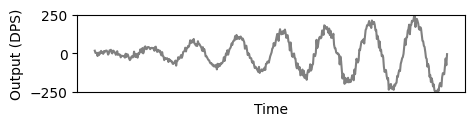
\includegraphics[width=\linewidth]{figure_scale_4.png}
            \label{fig_scale_4}
        \end{figure}
        \vspace{-8mm}

        The final result therefore retains the best characteristics of both sensors, range of sensor $A$ with noise-ratio of sensor $B$ (while possible).

    \pagebreak
    \subsection{Zero-rate}
        \subsubsection{Basis for calculations}
        \begin{itemize}
            \item The mean value of drift will be calculated by repeatedly integrating the expected drift on multiple axis and with multiple sensors, each of the axis and sensors adding additional variables to be integrated.
            \item To obtain realistic means, normal distribution will be factored in the calculations (see \ref{solution.rate.pdf}).
            \item The interval of the definite integrals is -1 to 1, since the negative part is important for making calculations in which opposing values cancel each other.
            \item To normalize the definite integration result from the (-1 to 1) interval to the (0 to 1) interval, the result must be divided by $ 2^N $, in which N is the number of needed integrations going into the negative side.
            \item The calculated zero-rate is a value from 0 to 1. The drift is a vector (in 1D, 2D or 3D) but only its length is relevant and the direction is irrelevant. That way the final integrated mean can be a simple scalar above zero.
            \item It is assumed that the zero-rate is many orders of magnitude smaller than the maximum detection range of the sensor, and therefore it will never reach its limits.
        \end{itemize}

        \subsubsection{Weighed probability}
        \label{solution.rate.pdf}
            Taking ($f_1$) "for any possible value of drift" and multiplying it for the adjusted normal distribution Probability Density Function ($f_2$), the resulting ($f_3$) provides "probability weighted drift" values allowing to perform calculations (and integrations) on it as if they were actual sensor output, but  also being able to obtain a realistic mean drift scalar (as perceived by the user), which will be the foundation for doing comparisons when adding more axis and more sensors.

            For the following figures, the arbitrary values for PDF sigma=0.3 and scale=0.75 will used to simulate a sensor with real world characteristics, but additionally a table with the final results for different PDF values will be shown too.
            \begin{figure}[H]
                \begin{center}
                    \caption{Probability-weighted drift}
                    \label{fig_rate_1a}
                    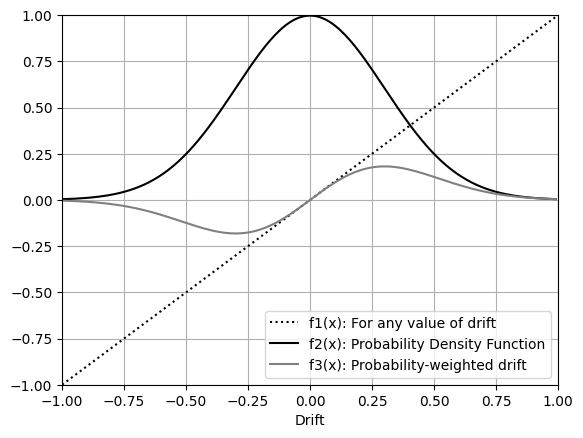
\includegraphics[width=0.8\linewidth]{figure_drift_1a.png}
                \end{center}
            \end{figure}
            $$ f_1(x) = x $$
            $$ f_2(x) = W(x) = pdf(x, \mu=0, \sigma=0.3) * 0.75 $$
            $$ f_3(x) = f_1(x)*f_2(x) $$

        \subsubsection{One axis}
            In figure \ref{fig_zero_11}, for a single axis and a single sensor, the mean can be integrated by using the absolute drift values.
            \begin{figure}[H]
                \begin{center}
                    \caption{Axis=1, Sensors=1}
                    \label{fig_zero_11}
                    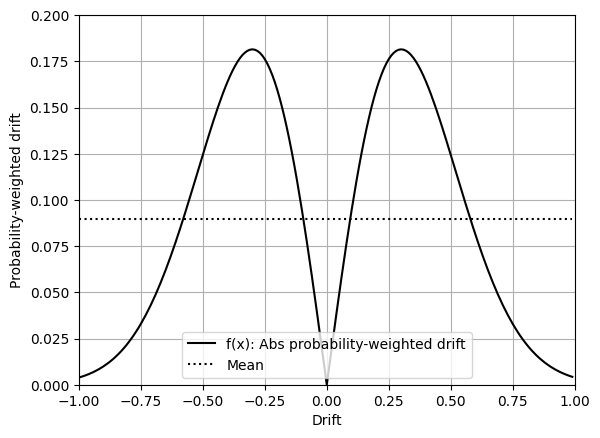
\includegraphics[width=0.8\linewidth]{figure_drift_1b.png}
                \end{center}
            \end{figure}
            \vspace{-8mm}
            $$ f(x) = |W(x)| $$
            $$ Mean = \frac{1}{2^1} \int_{-1}^1 |W(x)| dx = \int_0^1 W(x) dx \approx 0.0894 $$

            In figure \ref{fig_zero_12}, by adding a second sensor (also reporting on a single axis), values of both sensors can be averaged as $ (x_1 + x_2)/2 $, resulting in smaller mean drift.

            The negative part (interval $-1,1$) is used only until the point in which the goal is to start calculating absolute drift. This way an intermediate absolute() transformation between the 1st and 2nd integrations is not required.
            \begin{figure}[H]
                \begin{center}
                    \caption{Axis=1, Sensors=2}
                    \label{fig_zero_12}
                    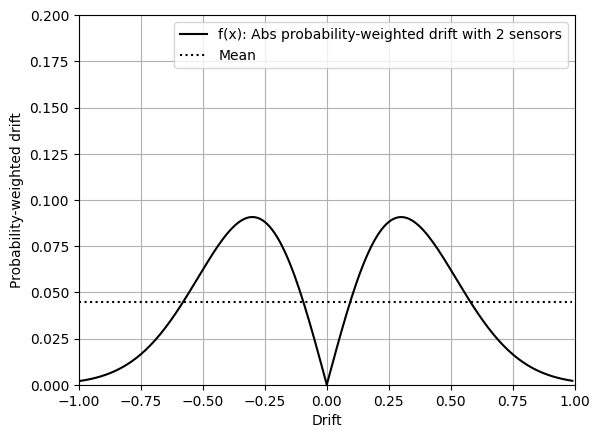
\includegraphics[width=0.8\linewidth]{figure_drift_2.png}
                \end{center}
            \end{figure}
            \vspace{-8mm}
            $$ f(x) = \left| \int \frac{ W(x_1) + W(x_2) }{2} dx_2 \right| $$
            $$ Mean = \frac{1}{2^1} \int_0^1 \int_{-1}^1 \frac{ W(x_1) + W(x_2) }{2} dx_1 dx_2  \approx 0.0447 $$

            So for a single axis, averaging the output of 2 sensors reduces the mean zero-rate to exactly half, independently of the values used to model the probability distribution.
            \begin{table}[H]
                \caption{Drift reduction on 1 axis}
                \vspace{2mm}
                \begin{tabular}{|r|r|r|r|r|}
                    \hline
                        PDF $\sigma$ & PDF scale & Sens=1 & Sens=2 & Reduction \\
                    \hline
                        0.2 &    1 & 0.0798 & 0.0399 & 0.5 \\
                        \textbf{0.3} & \textbf{0.75} & \textbf{0.0894} & \textbf{0.0447} & \textbf{0.5} \\
                        0.4 &  0.5 & 0.0763 & 0.0381 & 0.5 \\
                        0.5 & 1.25 & 0.0498 & 0.0249 & 0.5 \\
                    \hline
                \end{tabular}
            \end{table}

        \subsubsection{Two axis}
            In figure \ref{fig_zero_21}, when using 2 axis to create a 2-dimensional vector with length $\sqrt{x^2 + y^2}$ and direction $ atan2(x / y) $, and use PDF for both axis as described before.
            \begin{figure}[H]
                \begin{center}
                    \caption{Axis=2, Sensors=1}
                    \label{fig_zero_21}
                    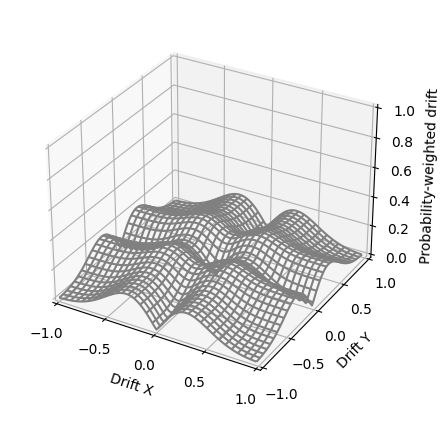
\includegraphics[width=0.8\linewidth]{figure_drift_3.png}
                \end{center}
            \end{figure}
            \vspace{-8mm}
            $$ f(x) = \sqrt{W(x)^2 + W(y)^2} $$
            $$ Mean = \frac{1}{2^2} \iint_{-1}^1 \sqrt{W(x)^2 + W(y)^2} dx dy \approx 0.1408 $$

            In figure \ref{fig_zero_22}, by using an additional sensor the probability-weighted drift is reduced overall, but specially depressed in the quadrants with opposing values (-,+) and (+,-).
            \begin{figure}[H]
                \begin{center}
                    \caption{Axis=2, Sensors=2}
                    \label{fig_zero_22}
                    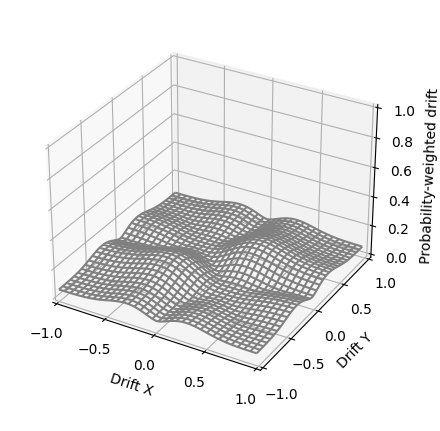
\includegraphics[width=0.8\linewidth]{figure_drift_4.png}
                \end{center}
            \end{figure}
            \vspace{-8mm}
            $$ U(a, b) = \frac{W(a)+W(b)}{2} $$
            $$
                f(x) = \iint \sqrt{
                    U(x_1, x_2)^2 +
                    U(y_1, y_2)^2
                } dx_2 dy_2
            $$
            $$
                Mean = \frac{1}{2^4} \iiiint_{-1}^1 \sqrt{
                    U(x_1, x_2)^2 +
                    U(y_1, y_2)^2
                } dx_1 dy_1 dx_2 dy_2
            $$
            $$ \approx 0.0982 $$

            \pagebreak
            So for 2 axis, used as 2-dimensional vectors, averaging the values of a 2nd sensor, it reduces the zero-drift to approximately $ \sim 2/3 $, varying depending on the characteristics of the sensor (the probability curve),

            This solution achieves better results when sigma is higher (when the drift is worse more often), while the scale used for the PDF is irrelevant.
            \begin{table}[H]
                \caption{Drift reduction on 2 axis}
                \vspace{2mm}
                \begin{tabular}{|r|r|r|r|r|}
                    \hline
                        PDF $\sigma$ & PDF scale & Sens=1 & Sens=2 & Reduction \\
                    \hline
                        0.2 & 1    & 0.1366 & 0.1033  & 0.7560 \\
                        \textbf{0.3} & \textbf{0.75} & \textbf{0.1407} & \textbf{0.0981} & \textbf{0.6972} \\
                        0.4 & 0.5  & 0.1137 & 0.07564 & 0.6655 \\
                        0.5 & 1.25 & 0.3165 & 0.2061  & 0.6511 \\
                    \hline
                \end{tabular}
            \end{table}

        \subsubsection{Conclusion}
            Redundant sensors can be used effectively to reduce zero-rate in ARS by exploiting the fact that for a set of given random vectors (with signed coordinates) their average is usually closer to the origin or coordinates than any of the individual vectors, or in the worst cases better than at least one of them.

            There are diminishing returns both when working with more axis (1D, 2D, 3D), and when adding more sensors.

            The same method could be also used with accelerometers to reduce zero-g, or with any other kind of sensor with similar random-walk bias characteristics.


\section{Methodology}
    \subsection{Calculations}
    The claims made in the solution section are backed by theoretical math, such calculations are formal explanations for the results obtained with real-life experimentation, and each result has been always cross-checked with other methods and tools.

    The main tool for calculations was NumPy, while also using Scipy Nquad or custom Montecarlo simulations to verify results.

    \subsection{About figures}
        Figures for noise (
            \ref{fig_noise_1},
            \ref{fig_noise_2},
            \ref{fig_noise_3},
            \ref{fig_noise_4},
            \ref{fig_noise_5}):
            Created using Numpy \textbf{np.random.normal} for emulating noise, and \textbf{np.random.seed} to operate over the same signals repeatedly. With length of $(\pi * 4)$ and resolution of (0.01). Plotted with Matplotlib.

        Figures for scale (
            \ref{fig_scale_1},
            \ref{fig_scale_2},
            \ref{fig_scale_3},
            \ref{fig_scale_4}):
            Created using Numpy \textbf{np.random.normal} for emulating noise, and \textbf{np.random.seed} to operate over the same signals repeatedly. With length of $(\pi * 16)$ and resolution of (0.1). Plotted with Matplotlib.

        Figures for zero-rate (
            \ref{fig_zero_11},
            \ref{fig_zero_12},
            \ref{fig_zero_21},
            \ref{fig_zero_22}):
            Created using Numpy and SciPy \textbf{scipy.stats.norm.pdf} to calculate Probability Density Distribution. Used \textbf{np.meshgrid} and \textbf{np.sum} for integrations. With Resolution of (0.01). Plotted with Matplotlib and wireframe for 3D.

    \subsection{Experimentation}
    The hypothesis about how to employ redundant sensors were originally tested with breadboard prototypes using a Raspberry Pi Pico and several pairs of IMUs such as 2x \emph{ST LSM6DS33}, 2x \emph{TDK MPU-6050}, and 2x \emph{Bosch BMX055}.

    Using these handmade devices as a computer \textbf{HID} input allowed to verify such hypothesis with ease, by emulating a mouse and having a real-time and interactive response to the sensors output.


\section{Potential applications}
    In the consumer electronics market, given the increased cost and diminishing returns in performance of using redundant IMUs, its application is possibly relegated to use-cases in which accuracy is a key factor, and enthusiasts are willing to cover the additional costs, such as videogame peripherals for e-sports, or high-performing/racing drones.

    In the medical field, redundant lower-grade sensors could be employed when industrial-grade sensors are too big or expensive, as for example electronic prosthetics.

    Even though this research is focused in lower-grade IMUs and computer input, the same methods could be used to combine data from multiple industrial-grade sensors and obtain extremely accurate data for scientific or industrial purposes.

\begin{thebibliography}{99}
    \bibitem{sensor_failure_detection}
        Merrill, Walter C.
        "Sensor failure detection for jet engines using analytical redundancy". Journal of Guidance, Control, and Dynamics.
        (1985).
        \url{https://doi.org/10.2514/3.20041}
    \bibitem{adaptive_kalman}
        Mohamed, A., Schwarz, K.
        "Adaptive Kalman Filtering for INS/GPS".
        Journal of Geodesy 73.
        (1999).
        \url{https://doi.org/10.1007/s001900050236}
    \bibitem{piezo_mems}
        Tadigadapa, S. A. K. M., and K. Mateti.
        "Piezoelectric MEMS sensors: state-of-the-art and perspectives"
        Measurement Science and technology.
        (2009).
        \url{https://doi.org/10.1088/0957-0233/20/9/092001}
    \bibitem{dtg}
        Bonfield, D. G.
        "The dynamically tuned gyroscope-A sensor for low cost attitude reference and navigation system".
        Applications of Modern Gyro Technology.
        (1977).
        \url{https://ui.adsabs.harvard.edu/abs/1977amgt.proc.....B}
    \bibitem{optical_mouse}
        Ng, Tuck Wah.
        "The optical mouse as a two-dimensional displacement sensor".
        Sensors and Actuators A: Physical 107.1.
        (2003).
        \url{https://doi.org/10.1016/S0924-4247(03)00256-5}
    \bibitem{zero_rate}
        Hiller, Tobias, et al.
        "Origins and mechanisms of bias instability noise in a three-axis mode-matched MEMS gyroscope".
        Journal of Microelectromechanical Systems 28.4.
        (2019).
        \url{https://doi.org/10.1109/JMEMS.2019.2921607}
\end{thebibliography}

\section*{Special thanks to}
\vspace{-2mm}
    Gu{\dh}ni Ólafsson.\\
    Michael Przybilski.

\end{document}




